\graphicspath{{content/chapters/5_design/figures/}}
\chapter{Desing}
\label{chp:design}

\section{System Design}
\label{sec:system_design}

The overall system design is modular, enabling seamless integration of different components and allowing for future extensibility. The system is divided into three main pipelines: training, denoising, and hyperparameter tuning. Each pipeline is implemented as a collection of functions with their respective parameters and outputs. These pipelines are coordinated through the \texttt{main.py} file, which serves as the entry point for the entire application.

All helper modules are organized under a \textit{Utils} folder, which contains essential functionality for dataset handling, model architecture definitions, training routines, denoising logic, and hyperparameter tuning. Additionally, a central configuration file, \texttt{config.py}, is located outside the \textit{Utils} folder near the \texttt{main.py} file. This file manages all the project’s parameters in the form of a dictionary, providing a centralized and easily modifiable interface. This approach enhances usability, allowing users to modify settings in one place and execute the pipeline directly through the main script.

A brief overview of the key files in the \textit{Utils} folder is provided below:

\begin{itemize}
    \item \texttt{dataset.py}: This file defines all dataset classes used in the project. These are implemented as PyTorch \texttt{Dataset} objects and support different strategies for handling variable-length audio inputs, as discussed in Section~\ref{sec:variable_length_handling}. This module also includes the definition of the \texttt{BucketSampler} class, which groups audio files of similar lengths to minimize padding and improve training efficiency. Additionally, it defines the \texttt{pto\_collate} function for batch collation and the \texttt{visualize\_dataset\_padding} function for visualizing the padding distribution in the dataset.
    
    \item \texttt{model.py}: This file defines all model architectures used in the project. Each model is implemented as a class inheriting from PyTorch’s \texttt{nn.Module}. Separating model definitions into their own module helps maintain a clean pipeline and facilitates experimentation with different architectures and hyperparameters.

    \item \texttt{train.py}: This file contains all functions related to model training, including the training loop, validation logic, and final evaluation. The training pipeline supports input from all three datasets defined in \texttt{dataset.py}, providing flexibility in training under different input-handling strategies. The modular design enables simple experimentation with alternative training setups and parameters.

    \item \texttt{denoise.py}: This module handles the denoising process and post-training evaluation. It follows a structure similar to the training pipeline but focuses on inference and metric computation. It supports both dataset-wide evaluation and single-sample inference. Additionally, this module allows the user to apply either of the two classical methods to the noisy input for comparison purposes, producing corresponding evaluation metrics.

    \item \texttt{classical.py}: This file implements traditional signal processing-based denoising algorithms used as baselines. These methods are implemented as standalone functions that take noisy waveforms as input and return denoised outputs. Where applicable, established libraries are used to implement these classical methods to avoid re-implementing known algorithms from scratch.

    \item \texttt{optuna.py}: This module handles hyperparameter tuning using the Optuna framework. It defines an optimization function that takes the training and validation datasets and returns the best-performing hyperparameter configuration. Due to the high memory requirements of certain models and datasets, this tuning pipeline is still being optimized for improved stability and efficiency.
\end{itemize}

\section{Variable Length Handling}
\label{sec:variable_length_handling}

For this project, only the clean and noisy pairs of audio files from the dataset are required — the transcript text files are ignored, as they are not relevant to the task. However, it is worth noting that such transcripts are highly valuable in other applications, such as training text-to-speech or speech recognition models.

As highlighted in the dataset analysis in Section~\ref{sec:dataset_exploration}, the audio files vary in length. This poses a challenge for model training, as batch processing requires input tensors to have consistent dimensions.

To address this, several algorithms for handling variable-length audio inputs were explored. The most basic approach involves padding each audio file to match the length of the longest sample in the batch, typically by appending zeros to the end of shorter files. While this method is simple, it has significant drawbacks: excessive padding introduces unnecessary data that may act as noise during training, making it harder for the model to learn effectively. The greater the variation in input lengths, the more padding is required — which can negatively impact overall training performance.

\begin{figure}[h]
    \centering
    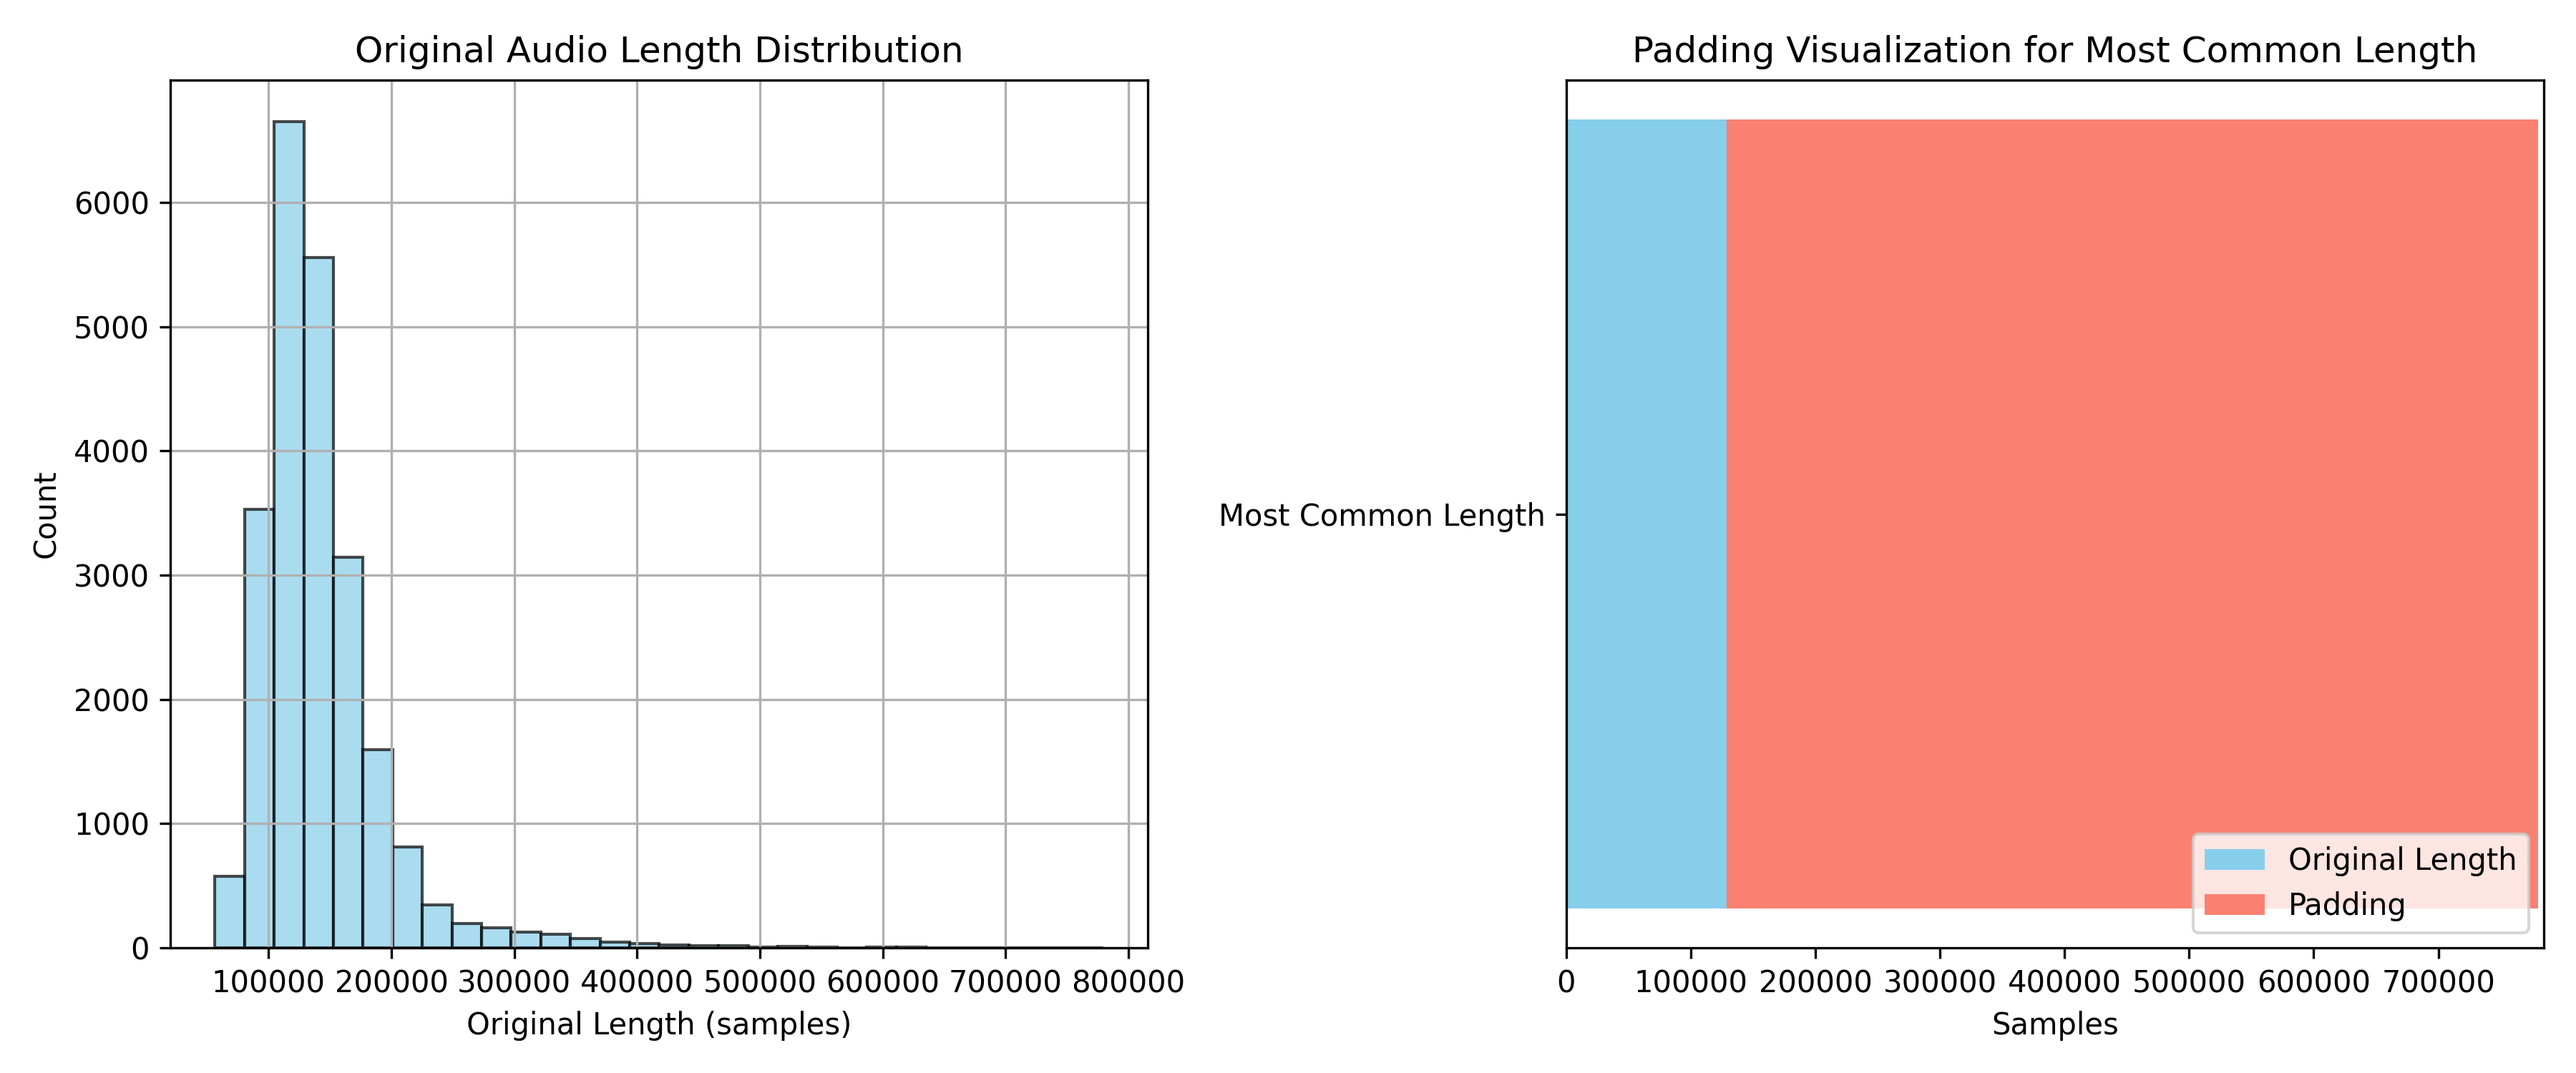
\includegraphics[width=\textwidth,keepaspectratio]{max_padding.png}
    \caption{\label{fig:max_padding}Illustration of maximum-length padding.}
\end{figure}

As shown in Figure~\ref{fig:max_padding}, the most common audio length is padded so heavily that the padding exceeds the actual content. This is far from ideal. To mitigate this issue, three different padding strategies were implemented. Each method aims to reduce the impact of excessive padding on model performance.

The first method is \textit{Static Bucketing}, which groups audio files into predefined fixed-length buckets. Building on this, the second method, \textit{Dynamic Bucketing}, creates buckets dynamically based on the distribution of audio lengths, offering a more adaptive grouping approach. The third and final method, inspired by a research paper~\cite{yoon2020pto}, proposes a simple, distortion-free technique for handling variable-length sequences through a combination of padding, truncation, and output truncation.

All three methods were implemented for testing and evaluation. Their role in the system design is critical, as they help ensure that the model can learn effectively without being hindered by dimensional mismatches or excessive zero-padding. Further details on the implementation of these methods are provided in Chapter~\ref{chp:implementation}, and their impact on model performance is discussed in Chapter~\ref{chp:evaluation}.

\section{Model Architecture}
\label{sec:model_architecture}

The model architecture is the highlight of the system design. It is the core component that determines how the system processes input data, how hidden layers and their connections are defined, and how the final output is generated. The modular design of the project as a whole facilitates the exploration of various model architectures. The main structure for speech enhancement models has already been introduced in Chapter~\ref{chp:literature_review}. With the concept of autoencoders being well-established in the literature, the most basic model defined in this work is a convolutional neural network (CNN) autoencoder.

\subsection{Convolutional Autoencoder (CNN)}

The CNN model implemented in this project serves as the baseline architecture. It is designed as a basic encoder-decoder model that operates directly on the real and imaginary components of the spectrogram, which are concatenated into a two-channel input. The encoder compresses the input using a series of convolutional layers and ReLU activations, reducing spatial dimensions while increasing the feature depth. A bottleneck layer captures the most salient features, followed by a decoder made of transposed convolutions that upsample the compressed representation back to the original shape.

The final output layer uses a \texttt{tanh} activation to constrain the values between -1 and 1, matching the typical range of normalized spectrogram values. The output is then split back into separate real and imaginary components. This basic structure allows the model to learn an end-to-end mapping from noisy spectrogram input to a denoised output while maintaining the shape consistency required for spectrogram inversion.

While simple, this model is critical for establishing a performance baseline and ensuring that the data pipeline, loss function, and inference process are correctly implemented.

\subsection{U-Net Architecture}

A U-Net is a type of convolutional neural network (CNN) commonly used for image segmentation tasks due to its effectiveness in preserving spatial information through skip connections. It is particularly well-suited for scenarios where both global context and fine-grained local detail are important — making it a strong candidate for spectrogram-based speech enhancement.

In this project, the U-Net architecture has been adapted to work with complex-valued spectrograms. Both the input and output consist of two channels representing the real and imaginary parts of the signal. The encoder compresses the input through multiple convolutional layers, each followed by group normalization and PReLU activations. The decoder performs the inverse operation using transposed convolutions, reconstructing the output with the help of skip connections from the encoder layers. These skip connections are aligned using bilinear interpolation to ensure matching dimensions, which is essential due to the varying spatial resolution after convolutional operations.

Compared to the basic CNN, the U-Net provides a deeper architecture with significantly better capacity for modeling both local patterns and long-range dependencies in the spectrogram. Its design allows for improved gradient flow and better reconstruction of fine detail in the denoised output.

\subsection{Conv-TasNet Architecture}

The Conv-TasNet is a convolutional, time-domain-based architecture originally proposed for speech separation. It avoids recurrence entirely by using stacked temporal convolutional networks (TCNs) to model long-term dependencies. In this project, the Conv-TasNet has been adapted for the frequency domain by operating on 2D spectrogram data, with two channels corresponding to the real and imaginary parts.

The architecture begins with an encoder that applies a convolutional transformation to the input spectrogram, projecting it into a higher-dimensional feature space. This is followed by a separation network composed of multiple stacks of dilated residual blocks, forming the TCN. These blocks use increasing dilation rates to capture long-range dependencies while maintaining efficient computation. Each residual block contains two convolutional layers, PReLU activation, and batch normalization, with residual connections ensuring stable gradient flow.

The decoder then transforms the processed features back into a two-channel spectrogram through another convolutional layer. To maintain shape consistency, both the residual blocks and the decoder truncate or interpolate the output as needed.

This architecture offers a high degree of temporal modeling while maintaining the advantages of convolutional efficiency. It serves as the most complex and expressive model evaluated in this project and is intended to compete with state-of-the-art enhancement techniques.

\subsection{Summary}

All three architectures were implemented within a unified framework that supports modular experimentation. Each model accepts and outputs two-channel spectrogram data, ensuring compatibility with the complex-valued processing pipeline. The CNN serves as a foundational benchmark, the U-Net balances performance with architectural elegance, and the Conv-TasNet pushes the boundary of what is achievable with convolutional architectures in this context. Their comparative performance and trade-offs are evaluated in Chapter~\ref{chp:evaluation}.


